\documentclass[11pt,letterpaper,titlepage]{article}
\usepackage[utf8]{inputenc}
\usepackage{graphicx}
\usepackage{tabu}
\usepackage{float}
\usepackage[toc,page]{appendix}
\usepackage{array}
\usepackage{layouts}

\usepackage[dvipsnames, table]{xcolor}
%\usepackage[style=ieee]{biblatex}
\usepackage{enumitem}
\usepackage[at]{easylist}
\usepackage{amsmath}
\usepackage{cleveref}
\usepackage{tabularx}
\usepackage{longtable}
%\usepackage{CJKutf8}
\usepackage{wrapfig}
\usepackage{textcomp}
\usepackage{pdfpages}
\usepackage{listings}
\usepackage{caption}
\usepackage{float}

\usepackage{amsfonts}
\usepackage{amssymb}
\usepackage{amsthm}
\usepackage{mathtools}
\usepackage[margin=2.5cm]{geometry}
\DeclarePairedDelimiter{\ceil}{\lceil}{\rceil}
\geometry{portrait, margin=2.5cm}
	
\title{ROB313 Report}
\author{Zhengmin Yang}
\date{\today}


\begin{document}
	\maketitle
	
	\section{Introduction}
	\paragraph{Objectives}
	In this report we will explore the application of gradient descent to modelling classification problems using machine learning. Both binary classification and multiclass classification will be considered. For binary classification, the prediction function is a sigmoid function (1) and the negative log likelihood, which is also the loss function, is given (2).
	\begin{equation}
	sigmoid(x)=\frac{1}{1+e^{x}}
	\end{equation}
	\begin{equation}
	\log Pr(\boldmath y \unboldmath | \boldmath w \unboldmath, \boldmath X \unboldmath)  = \sum_{i=1}^{N} y^{(i)}\log(\hat{f}(\boldmath x^{(i)}\unboldmath; \boldmath w \unboldmath)) + (1-y^{(i)})\log (1-\hat{f}(\boldmath x^{(i)} \unboldmath; \boldmath w \unboldmath))
	\end{equation}
	
	Note that the log likelihood will equal $-\infty$ if the predicted class probability is $\hat{f}(\boldmath x^{(i)}; \boldmath w) = 1$ but the actual label is 0. This means that the model is telling us that the class is not 0 with 100\% confidence although it is 0. This makes sense from a mathematical perspective. We are trying to maximize the likelihood of making a correct prediction, i.e. the log likelihood. Since this prediction is completely incorrect, it is in our best interest not to choose it. With a value of $- \infty$ this ensures that when we apply the argmax function we will never choose the value of w that gave us this completely incorrect prediction.
	
	For multiclass classification, the prediction function is the softmax function (3) and the negative log likelihood (loss function) is given by (4).
	\begin{equation}
	softmax(x_{j})=\frac{e^{x_{j}}}{\sum_{i=1}^{K}e^{x_{i}}}
	\end{equation}
	\begin{equation}
	\log Pr(\boldmath Y \unboldmath | \boldmath X \unboldmath, \boldmath w \unboldmath) = \sum_{i=1}^{N} \sum_{j=1}^{K}  y_{j}^{(i)}\log(\hat{f_{j}}(\boldmath x^{(i)} \unboldmath,\boldmath w \unboldmath))
	\end{equation}
	
	Both full batch gradient descent and SGD utilize the fact that we are able to minimize the loss with respect to the weights $\boldmath w$ by moving the weights in a direction opposite the gradient of the loss (with respect to the weights). The amount that we move by can be calculated by using a line search algorithm (included in the file submission but not used) or set as a parameter $\eta$, also known as learning rate (used for this assignment). The weight update at the (k+1)th iteration is given by the following:
	\begin{equation}
	\boldmath w^{(k+1)} \unboldmath = \boldmath w^{(k)} \unboldmath - \eta \triangledown \log Pr(\boldmath y \unboldmath | \boldmath w^{(k)} \unboldmath, \boldmath X \unboldmath)
	\end{equation}
	
	\section{Binary Classification}
	\subsection{Full Batch Gradient Descent for Binary Classification}
	Full batch gradient descent uses the entire set of training data as inputs to the loss function to calculate the direction to move the weight vector. The following figure shows losses with three different learning rates.
	\begin{figure}[H]
		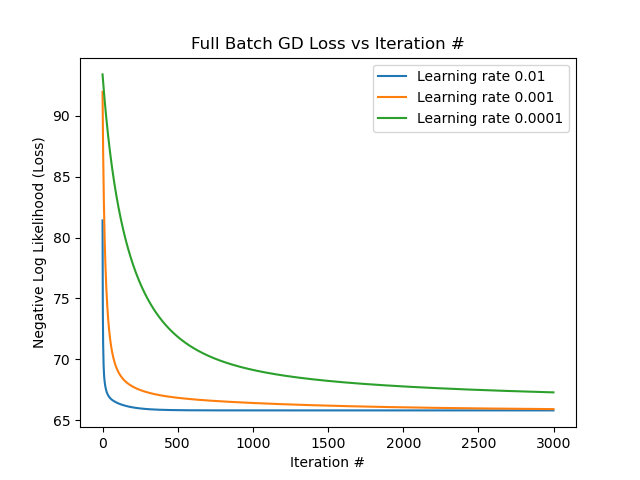
\includegraphics[width=\linewidth]{Full Batch GD.png}
		\caption{Loss for varying values of $\eta$.}
		\label{fig:Full Batch GD}
	\end{figure}
 	As we can see, the learning rate of 0.01 corresponds to the smallest loss. The largest testing accuracies correspond to learning rates of 0.01 and 0.0001, and the smallest testing loss corresponds to the largest learning rate, 0.01. This correlates well with the trends set by the training loss, which indicates that a slower learning rate corresponds to a larger loss is therefore more inaccurate. This is because a smaller learning rate corresponds to a slower convergence, as seen in the graph.
 	For example, a learning rate of 0.01 allows the loss to converge very quickly at roughly the 200th iteration. However the loss converges slower for a learning rate of 0.001, at around the 2500th iteration, while the loss has yet to converge at the 500th iteration for a learning rate of 0.0001. This makes sense because the learning rate corresponds to the step size that we take every time we update the weight vector; a larger step size results in a faster descent towards a minimum and hence a faster convergence rate.
 	
	\begin{tabular}{|l|l|l|l|}
		\hline
		Learning Rate & Testing Accuracy & Testing Loss & Training Loss \\ \hline
		0.01          & 0.733            & 6.91         & 65.8          \\ \hline
		0.001         & 0.667            & 7.00         & 66.8          \\ \hline
		0.0001        & 0.733            & 7.06         & 77.9          \\ \hline
	\end{tabular}
 	\captionof{table}{Testing Accuracy, Testing Loss, and Training Loss for Different Learning Rates}\label{Full Batch GD}
 	
	
	
	\subsection{Stochastic Gradient Descent for Binary Classification}
	Stochastic Gradient Descent differs from Full Batch Gradient Descent in that it randomly chooses a training point as an input to the loss function in order to find the gradient. Because of this random process, the loss curves that it generates are jagged. It can be shown that SGD is an unbiased estimator of the full batch gradient descent despite being less expensive computationally. The results below agree heuristically with the results previously obtained by using full batch gradient descent.
	\begin{figure}[H]
		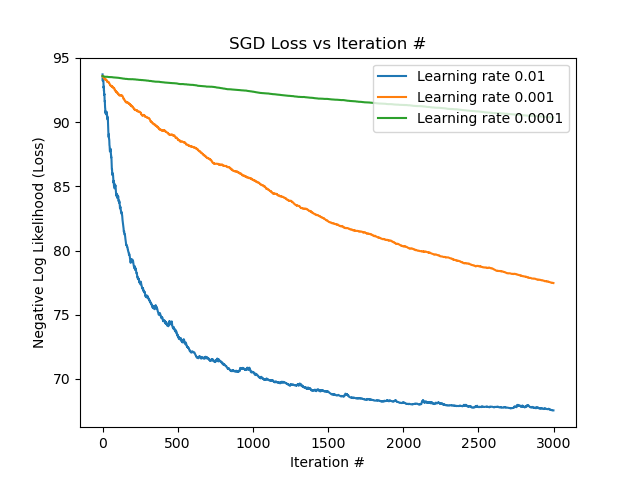
\includegraphics[width=\linewidth]{SGD.png}
		\caption{Loss for varying values of $\eta$.}
		\label{fig: Stochastic GD}
	\end{figure}
	Again, this confirms that the learning rate of 0.01 corresponds to the smallest training loss. The highest testing accuracies correspond to learning rates of 0.01 and 0.001 while the lowest testing loss corresponds to the highest learning rate like in full batch gradient descent. This also correlates directly with the convergence rates of the loss function. For example, we can see that the loss corresponding to a learning rate of 0.01 shows signs of convergence after about the 2000th iteration, while the losses for the other two learning rates are still converging and do not show any sign of convergence even after the 300th iteration. Judging by the shapes of the curves it is apparent that the curve corresponding to a learning rate of 0.001 is moving towards convergence faster than the curve corresponding to a learning rate of 0.01.
	
	\begin{tabular}{|l|l|l|l|}
		\hline
		Learning Rate & Testing Accuracy & Testing Loss & Training Loss \\ \hline
		0.01          & 0.733            & 6.79         & 67.9          \\ \hline
		0.001         & 0.733            & 8.33         & 76.5          \\ \hline
		0.0001        & 0.667            & 10.0         & 90.4          \\ \hline
	\end{tabular}
	\captionof{table}{Testing Accuracy, Testing Loss, and Training Loss for Different Learning Rates}\label{SGD}
	
	\subsection{Comparison Between Full Batch GD and SGD}
	\subsubsection{Convergence Rates}
	Full batch gradient descent (FBGD) converges a lot faster than SGD in terms of the number of iterations performed. However due to the fact that we use all of the training data to compute the gradient it is more computationally expensive than SGD. This tradeoff is not apparent in small datasets such as this, where the time to run the models is roughly the same (around 0.4 seconds per model) but will become apparent in larger datasets where FBGD's computation time will slow down dramatically due to the dependence of its computation on the size of the dataset. SGD on the other hand, while converging in a higher number of iterations will run faster due to its computational independence on the size of the dataset.
	\subsubsection{Losses}
	FGBD and SGD present similar losses for learning rates of 0.01 and 0.001, suggesting that SGD is a good estimator of FBGD while being less computationally expensive. In addition, as sjhown in class, the expected value of an SGD update is equivalent to an FBGD update, again confirming their similarities. They show different results for learning rate = 0.0001 because the SGD loss has not yet converged and did not show any sign of convergence. Thus SGD's training loss is much higher than FBGD's.
	\subsection{Test Log Likelihood as a Metric}
	The testing log likelihood could be a more suitable metric than test accuracy for measuring performance. This is because the signmoid gives a range of probabilities, which is then mapped to one class or another. The probabilities could be thought of as confidences in whether an input belongs to a certain class. However the testing accuracy loses this confidence information when it maps the outputs of the sigmoid onto a class. By using the log likelihood we are also able to determine whether the model its confidence in giving the correct output in addition to whether is really giving the correct output. 
	\section{Stochastic Gradient Descent for Multiclass Classification}
	
	
	
\end{document}